
%===========================================================
\section{Algorithm} 
\label{section:systemoverview}
   
   In this section, we introduce our hierarchically fused fully convolutional network (HF-FCN) for extracting rooftops, and the implementation in the training stage.
    
%We directly learn a mapping from raw pixels in $\mathbf{S}$ to a true label image  $\mathbf{\tilde{M}}$ by training the whole network. Fig. \ref{fig:AGroupOfExamples} shows an example of $\mathbf{S}$, $\mathbf{\tilde{M}}$, $\mathbf{\hat{M}}$. Here we formulate our approach for building extraction.
    
\subsection{Network Architecture}  
  Given an input aerial image $\mathbf{S}$, our goal is to predict a label image $\mathbf{\hat{M}}$ where 1 for the pixel belonging to a building and 0 otherwise. We use similar strategy with semantic segmentation. 
  We modify the VGG16 Net~\cite{Simonyan2015Very} by hierarchically fusing the response of all layers together, as shown in Fig. \ref{fig:hierarchicalFCN}. 
  The VGG16 Net~\cite{Simonyan2015Very} has 16 convolutional layers and five 2-stride down-sampling layers, from which we can acquire enough multi-level information. Its network parameters pre-trained on ImageNet are helpful for initializing our network  because our aerial data are essentially optical imagery. 
  We made the following modifications to detect buildings more effectively. 
  Firstly, the sixth and seventh fully connected layers and the fifth pooling layer in VGG16 Net are cut, because they are at $1/32$ of the resolution of the input image. 
  As a result, the interpolated prediction map will be too fuzzy to utilize. Meanwhile, the number of neurons in the sixth and seventh convolutional layers is too large to cost intensive computation. 
  The trimmed VGG16 Net is denoted as Level 1 in our HF-FCN.
    %
  Secondly, the feature map from each convolutional layer in Level 1 are fed into a convolutional layer with a filter of $1\times1$ kernel. The outputs of these convolutional layers are upsampled and cropped to the size of input image. 
  Upsampling is implemented via deconvolution which is initialized by bilinear interpolation.  
  These upsampled feature maps compose the Level 2 in our HF-FCN. 
  %
  Finally, all the feature maps in Level 2 are stacked and put into a convolutional layer with a filter of kernel size of 1$\times$1  to yield final predicted map, denoted as Level 3 in our HF-FCN. 
  %
  The size of the feature map in last stage of Level 1 is $1/16$ of input image, which is too small to use. 
  Thus, the input images are padded with all-zero band to enlarge the size of feature maps, similar as  \cite{Long2014Fully}. 
 
\begin{figure}
\centering
\includegraphics[width=95mm]{figs/hierarchicalFCN-revision}
\caption{Our network architecture. F$1\_1$ means the fusion of feature maps generated from its corresponding convolutional layer conv$1\_1$, U$1\_1$ means the upsampling of F$1\_$1, and so forth.}
\label{fig:hierarchicalFCN}
\end{figure}

   \begin{table}	
	\centering 
	\caption{The receptive field (RF) and the stride size of Level 2 in our architecture.}	
 	\begin{tabular}{C{1cm}|*{16}{C{0.74cm}}} 
	\hline
	layer & F1$\_$1 & F1$\_$2  & F2$\_$1  & F2$\_$2  & F3$\_$1  & F3$\_$2  & F3$\_$3  & F4$\_$1  &   F4$\_$2  & F4$\_$3  & F5$\_$1 & F5$\_$2  &F5$\_$3 \\
	\hline
    RF & 3 & 5  & 10 & 14  & 24  & 32  & 40  & 60  & 76  & 92 & 124  & 164  & 196 \\
	\hline
	stride & 1 & 1   & 2  & 2  & 4  & 4  & 4  &8  & 8  & 8  & 16  & 16  & 16 \\
	\hline
    \end{tabular}
    \label{tab:receptivefield} 
   \end{table}         
    
   In Level 2, the feature maps with increasing receptive field (see Table \ref{tab:receptivefield}) capture local information in larger neighbourhood sizes at higher semantic levels. The shallow layers generate feature maps with fine spatial resolution but low level semantic information. In contrast, the deep layers generate coarse feature maps with high-level semantic information. The feature maps at middle layers correspond to certain intermediate-level features. Integrating all these feature maps, buildings with variant appearances or occlusions are effectively extracted.
  An example is shown in Fig.~\ref{fig:featuremapsofHF-FCN}. Given an aerial image, the U$1\_$1 in Fig. \ref{fig:featuremapsofHF-FCN}(b) with small receptive field extracts low-level features like edges and corners. In Fig.~\ref{fig:featuremapsofHF-FCN}(c), the U1$\_$2 functions like an over-segmentation which groups pixels with similar color or texture into a subregion. 
  In the U2$\_$1 as Fig.~\ref{fig:featuremapsofHF-FCN}(d) shows, shape information is augmented. 
  From the U3$\_$3 as Fig.~\ref{fig:featuremapsofHF-FCN}(e) shows, we can see that regions with significantly varying appearances are merged into an integrated building by considering high-level features. In U4$\_$2 and U5$\_$2 (see Fig.~\ref{fig:featuremapsofHF-FCN}(f)(g)), our network learns strong semantic knowledge to distinguish dark rooftops with dim shadows and dark-green water area. In Level 3, we show that HF-FCN obtains a reliable prediction by combining multi-level semantic information and spatial information, as Fig.~\ref{fig:featuremapsofHF-FCN}(h) shows. 

\begin{figure}
\centering
\includegraphics[width=120mm]{figs/featuremaps}
\caption{(a) Input aerial image. (b - g) Feature maps generated from U1$\_$1, U1$\_$2, U2$\_$1, U3$\_$3, U4$\_$2, U5$\_$2, respectively. (h) Predicted labelling map.}
\label{fig:featuremapsofHF-FCN}
\end{figure}

%   In VGG16 Net, 
%   For instance, the first stage generate low level semantic information, such as, regions with similar color or texture, and fine spatial resolution. On the contrary, the last stage outputs strong semantic features but coarse map
%   
%   There are three reasons that FCN-8s is not appropriate methods for building extraction. (1) \textbf{The output of 32 stride layers, including convolutionalized \textit{fc6, fc7} and fifth pooling layer, } (2) The output from FCN-8s is at one-eight of the input resolution. It is not dense enough for very high resolution remote sensing image. Though FCN4s and FCN2s can increase the resolution, they have little help for improving performance. Defective fusion strategy is the most likely reason. On the one hand, in \cite{Long2014Fully}, the coarse predictions from a late stage are upsampled and combined with prediction from its preceding stage using simple sum operation. (3) \textbf{ For instance, in FCN-8s,
%   
% There are two main considerations for choosing hierarchy architecture. Firstly,  buildings especially with large-size have variant appearancess or occlusions.   
   
%\subsection{Architecture Alternatives} 
%In this section, we firstly introduce a well-known semantic segmentation network, called fully convolutional network(FCN)\cite{Long2014Fully}. We attempt to extract footprints of building  using  architecture proposed by author and two modified versions. Our experiments show that these networks are not enough to accomplish building  extraction task. 
%	In our experiments, we first directly apply the FCN-8s to extract building rooftop by replacing the loss function with sigmoid cross-entropy loss. In order to achieving better performance, the network is extended to FCN-4s, FCN-2s. Our experiments show that FCN-4s and FCN-2s get the best performance with overall recall of 70.19 $\%$ in precision recall breakeven point. According to our results, the first row of Fig. \ref{fig:FCN4s-results} indicates that FCN-4s has less ability to handle  objects with small size. The second row of Fig. \ref{fig:FCN4s-results} shows that it is hard for FCN to discriminate buildings with ground if their color is similar. To overcome these drawbacks, a improved FCN is introduced in next section. 
%	
%\begin{figure}
%\centering
%\subfigure[]{	
%	\label{fig:InputImage}
%	\includegraphics[width=35mm]{FCN4s-results-Input(a)}}
%\subfigure[]{
%	\label{fig:GroundTruth}
%	\includegraphics[width=35mm]{FCN4s-results-GT(b)}}
%\subfigure[]{
%	\label{fig:FCN-4s}
%	\includegraphics[width=35mm]{FCN4s-results-Prediction(c)}}
%\subfigure[]{	
%	\label{fig:InputImage}
%	\includegraphics[width=35mm]{FCN4s-results-Input(d)}}
%\subfigure[]{
%	\label{fig:GroundTruth}
%	\includegraphics[width=35mm]{FCN4s-results-GT(e)}}
%\subfigure[]{
%	\label{fig:FCN-4s}
%	\includegraphics[width=35mm]{FCN4s-results-Prediction(f)}}
%\caption{(a)(d) Input image. (b)(e) Ground truth. (c)(f) FCN-4s prediction.}
%\label{fig:FCN4s-results}
%\end{figure}
% 
        
\subsection{Network Training}
   
 In the training stage, we train our network to directly generate a prediction map $\mathbf{\hat{M}}$ from raw pixels in the input aerial image $\mathbf{S}$ to approach a true label image $\mathbf{\tilde{M}}$. 
 Fig.~\ref{fig:AGroupOfExamples} shows an example of $\mathbf{S}$, $\mathbf{\tilde{M}}$, $\mathbf{\hat{M}}$.  
  %
   We denote our input training data set as $\mathbf{I} = \{(\mathbf{S}_{i},\mathbf{\tilde{M}}_{i}),i = 1,\ldots,N\}$, $N$ is the number of aerial image and labeled map pairs.
% where sample $\mathbf{S}_{n} = \{s_{j}^{(n)}, j = 1,\ldots,\vert \mathbf{S}_n \vert \}$ denotes the raw input image and  $\mathbf{\tilde{M}}_{n} = \{\tilde{m}_{j}^{(n)}, j = 1,\ldots,\vert \mathbf{S_n} \vert\}$, $\tilde{m}_j^{(n)} \in \{0,1\}$ denotes the corresponding ground truth binary labelling map for satellite image $\mathbf{S}_{n}$.  
Taking account of each input image holistically and independently, the subscript $i$ is ignored  for notational simplicity in the following definition. 
In our image-to-image training stage, the loss function is computed over all pixels in a training image $\mathbf{S} = \{s_{j}, j = 1,\ldots,\vert \mathbf{S} \vert\}$ and building map $\mathbf{\tilde{M}} = \{\tilde{m}_{j}, j = 1,\ldots,\vert \mathbf{S} \vert\}$, $\tilde{m}_j \in \{0,1\}$, where $|S|$ is the number of pixels in $\mathbf{S}$.
%
For simplicity, we denote the collection of all standard network layer parameters as $\mathbf{W}$. For each pixel $j$ in a training image, the probability that assigns it to building is denoted as its probability as a building $\hat{m}_j$. 
We use the sigmoid cross-entropy loss function defined as 
\begin{equation}
	\label{loss}
    \mathcal{L} = - \frac{1}{\vert \mathbf{S} \vert} \sum_{s_j \in \mathbf{S}} \left[ \tilde{m}_j \log{\hat{m}_j} + (1 - \tilde{m}_j)\log{(1 - \hat{m}_j)} \right].
\end{equation}

%\begin{figure}
%\centering
%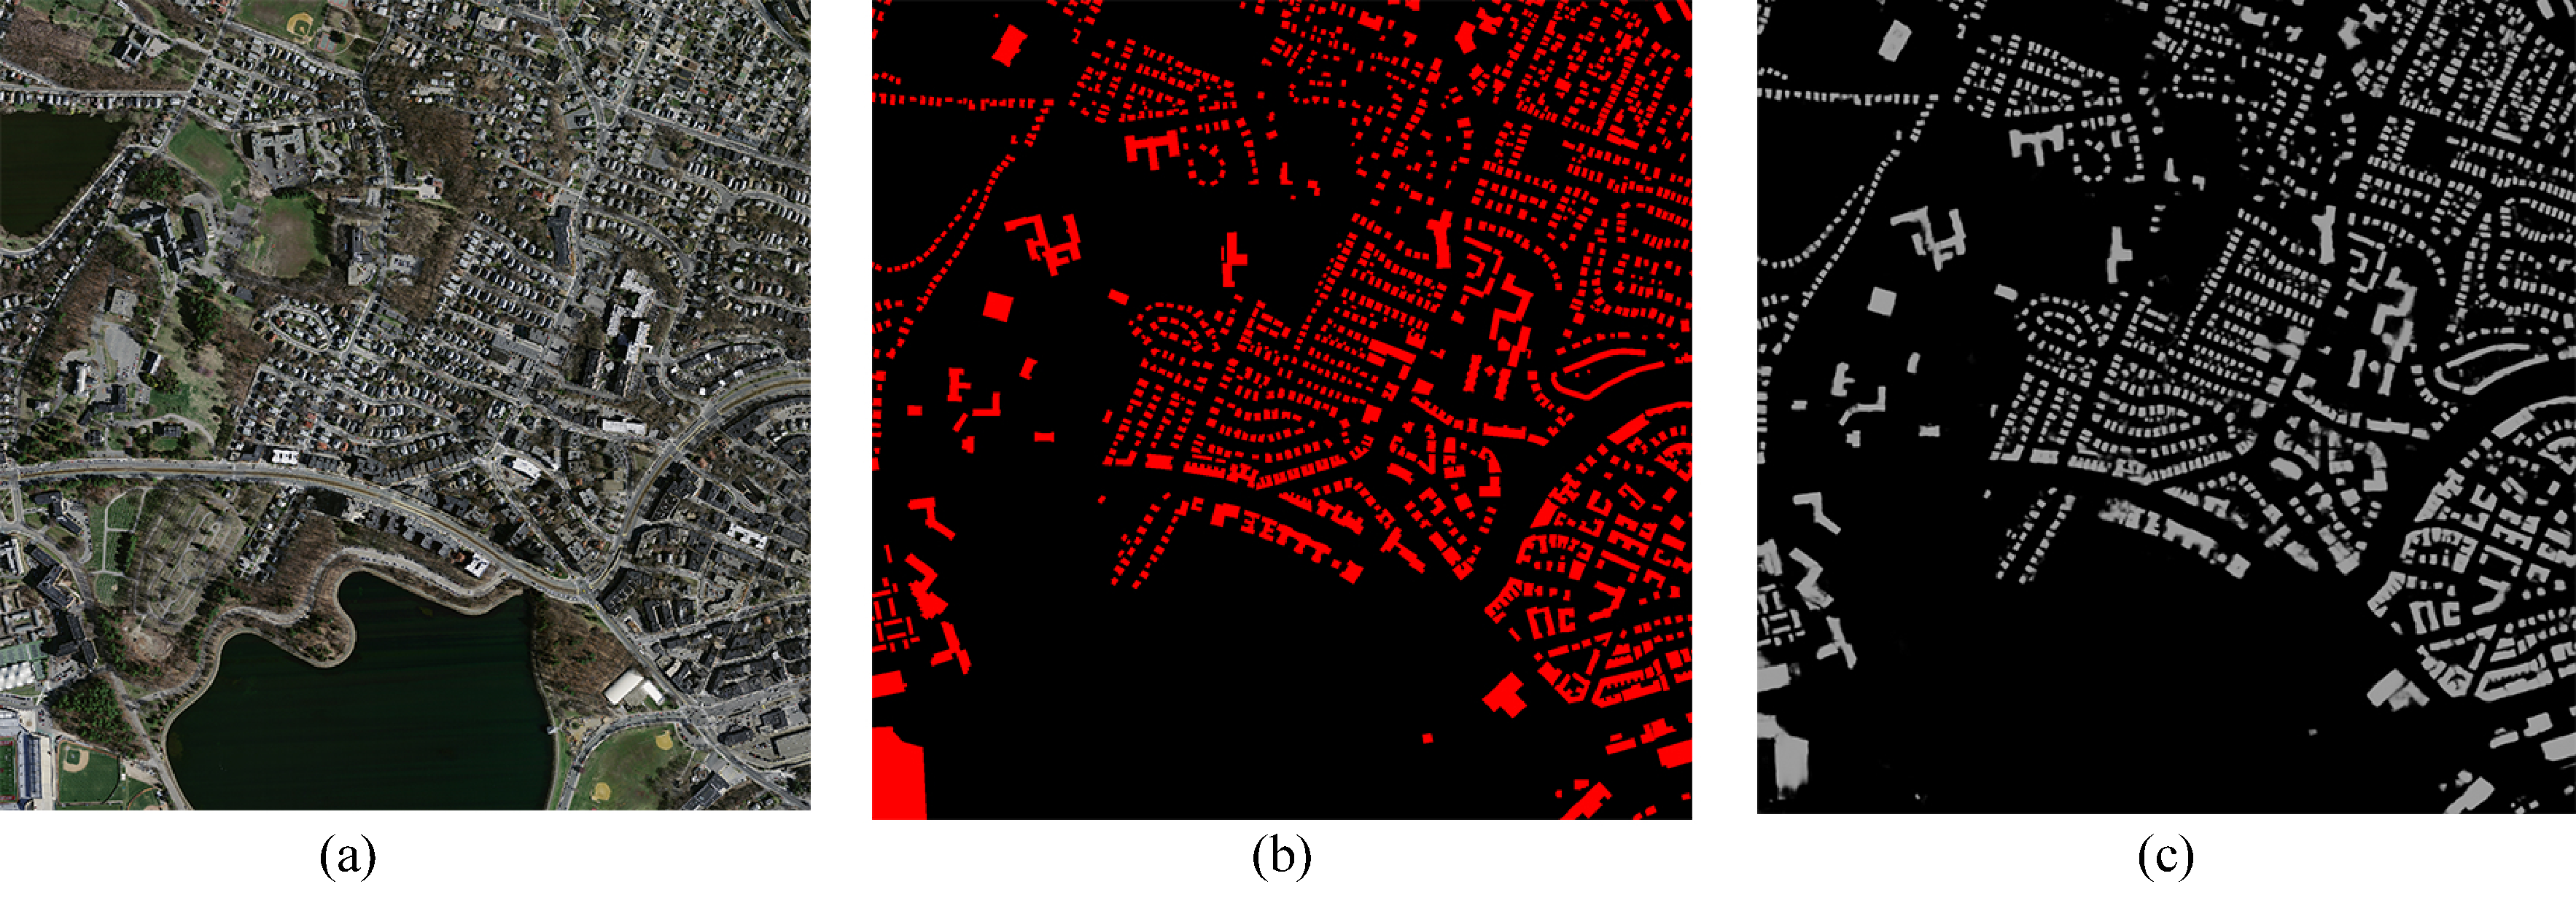
\includegraphics[width=120mm]{AGroupOfExamples}
%\caption{(a) Aerial image $\mathbf{S}$. (b) Ground truth $\mathbf{\tilde{M}}$. (c) Predicted label image $\mathbf{\hat{M}}$. }
%\label{fig:AGroupOfExamples}
%\end{figure}

\begin{figure}
\centering
\subfigure[Aerial image $\mathbf{S}$]{	
	\label{fig:AerialImage}
	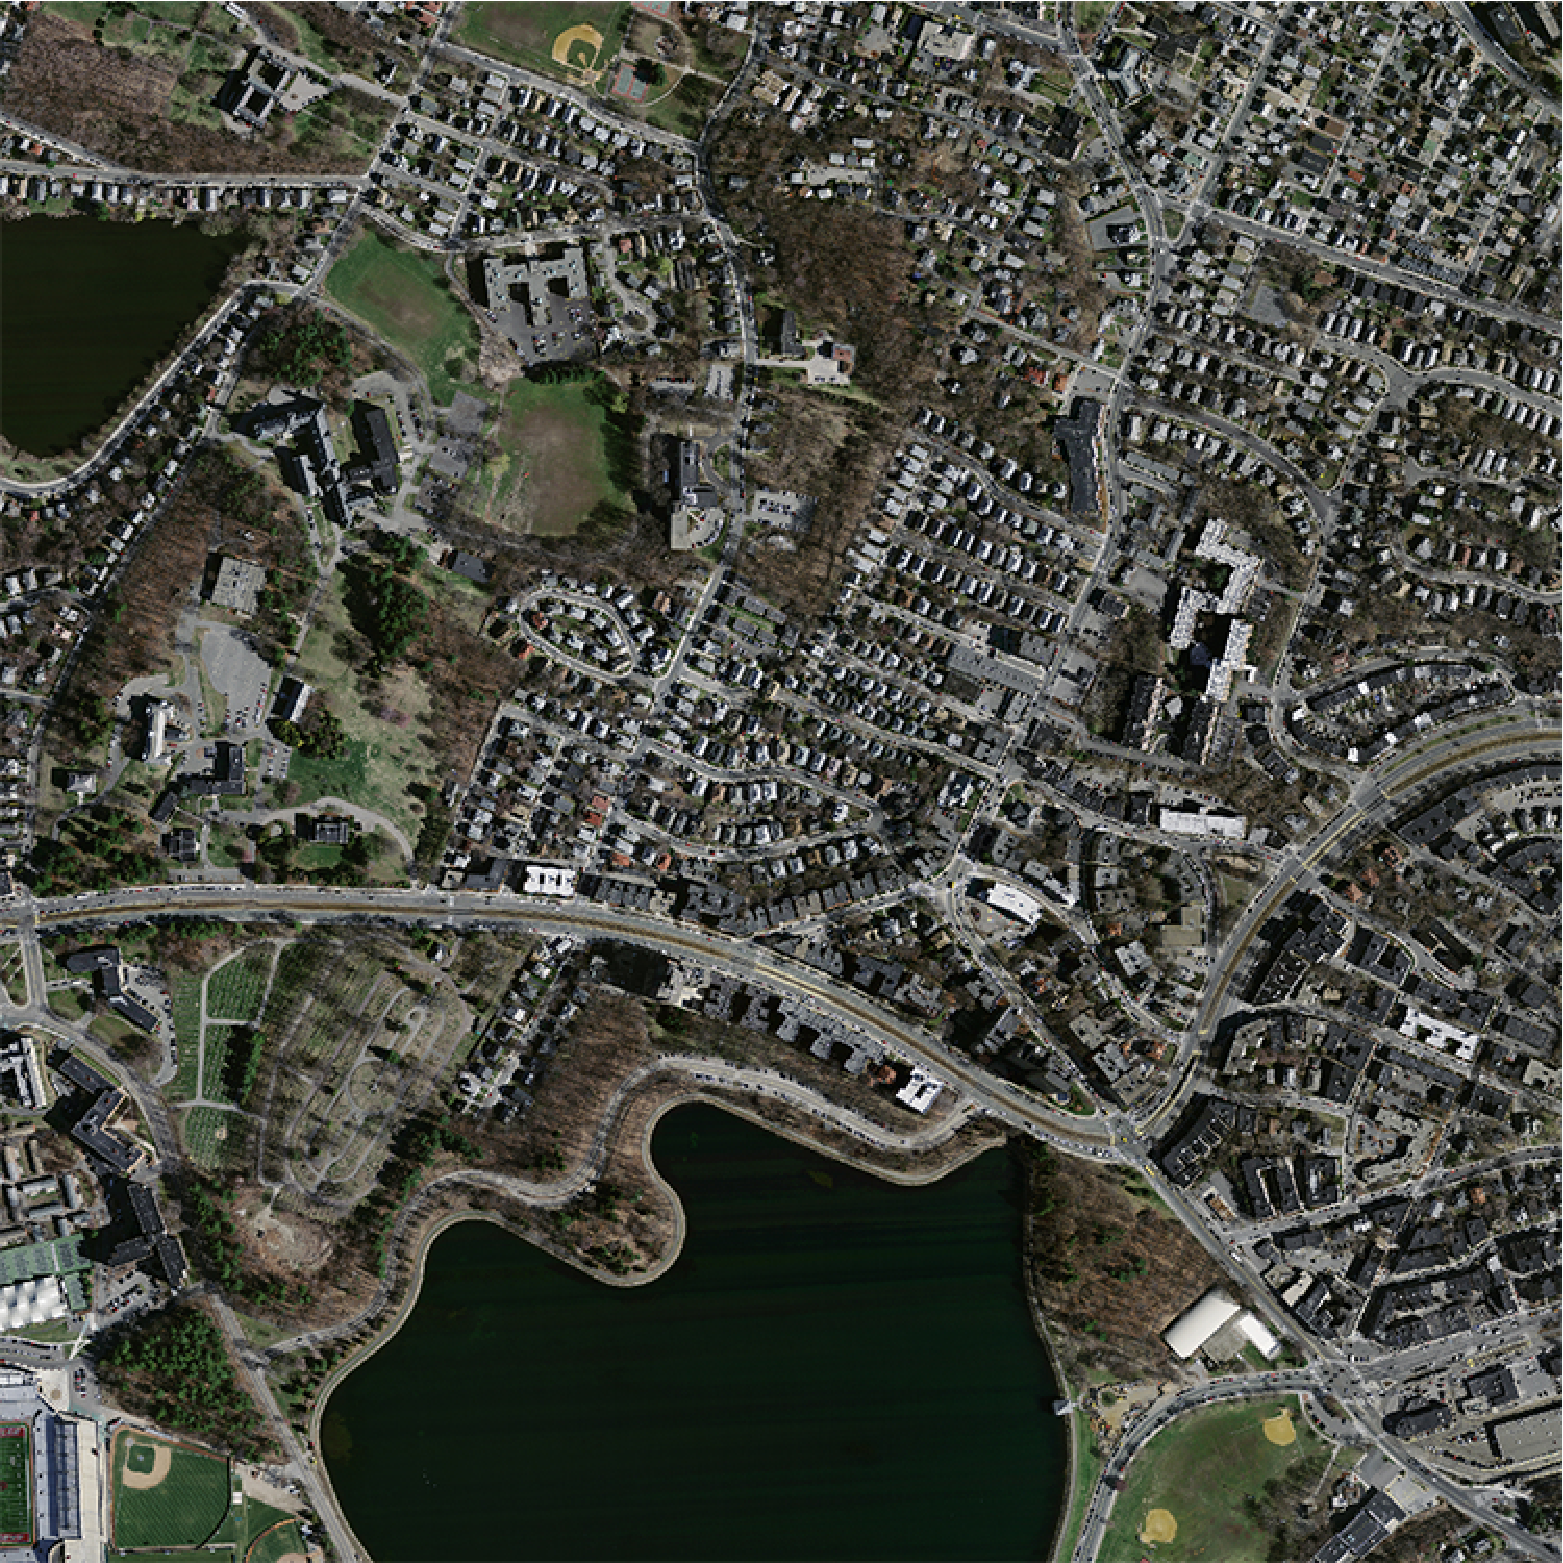
\includegraphics[width=38mm]{figs/example-aerialImage}}	
\subfigure[Ground truth $\mathbf{\tilde{M}}$]{
	\label{fig:GroundTruth}
	\includegraphics[width=38mm]{figs/example-GT}}	
\subfigure[Predicted image $\mathbf{\hat{M}}$]{
	\label{fig:PredictedResutls}
	\includegraphics[width=38mm]{figs/example-prediction}}	
\caption{ An example of the resulting predicted image.}
\label{fig:AGroupOfExamples}
\end{figure}

